\PassOptionsToPackage{utf8}{inputenc}
\documentclass[12pt]{report}

\usepackage[margin=2cm]{geometry}

\usepackage{graphicx}

\renewcommand{\thefigure}{S\arabic{figure}}

\begin{document}

\begin{figure}[b]
	\centerline{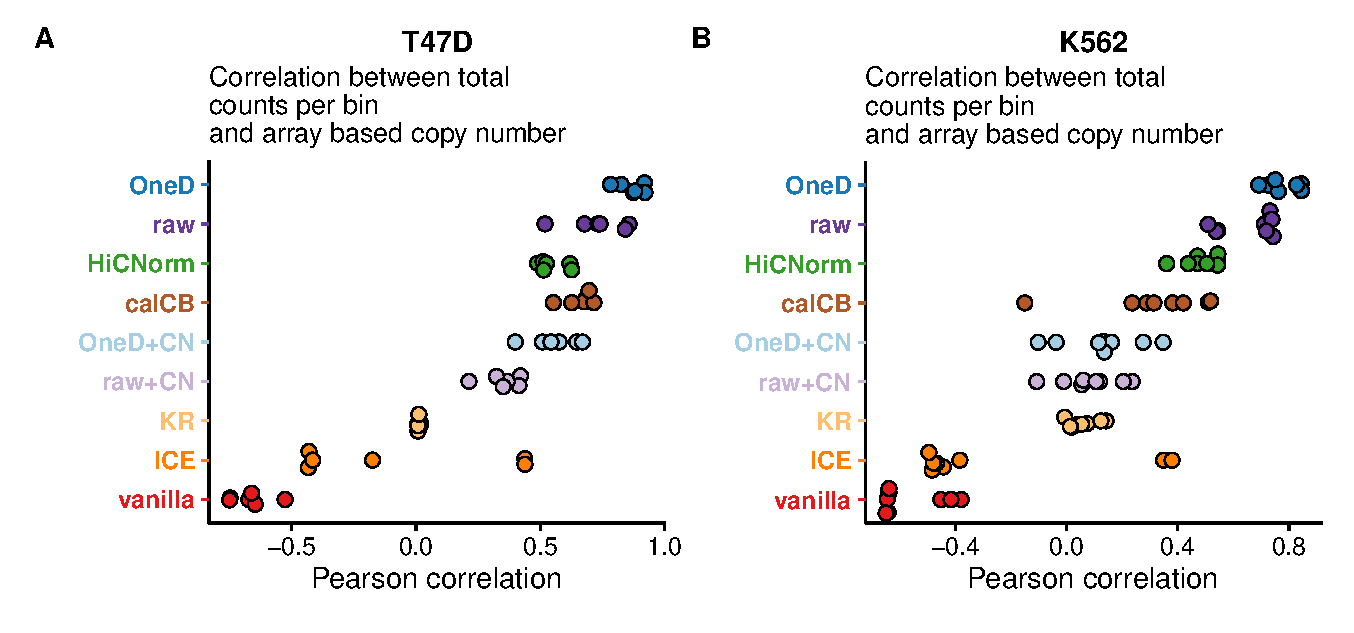
\includegraphics[width=\textwidth]{nar_figures/supp_figure_1.eps}}
	\caption{
    Pearson correlation between contact profiles and independent copy number
	estimation (COSMIC). A. T47D breast cancer cell line (6 samples). B. K562
	leukemia cell line (8 samples). Each dot represents a sample. The new
	proposal (in dark blue) outperforms the rest of alternatives.}
\end{figure}

\begin{figure}
	\centerline{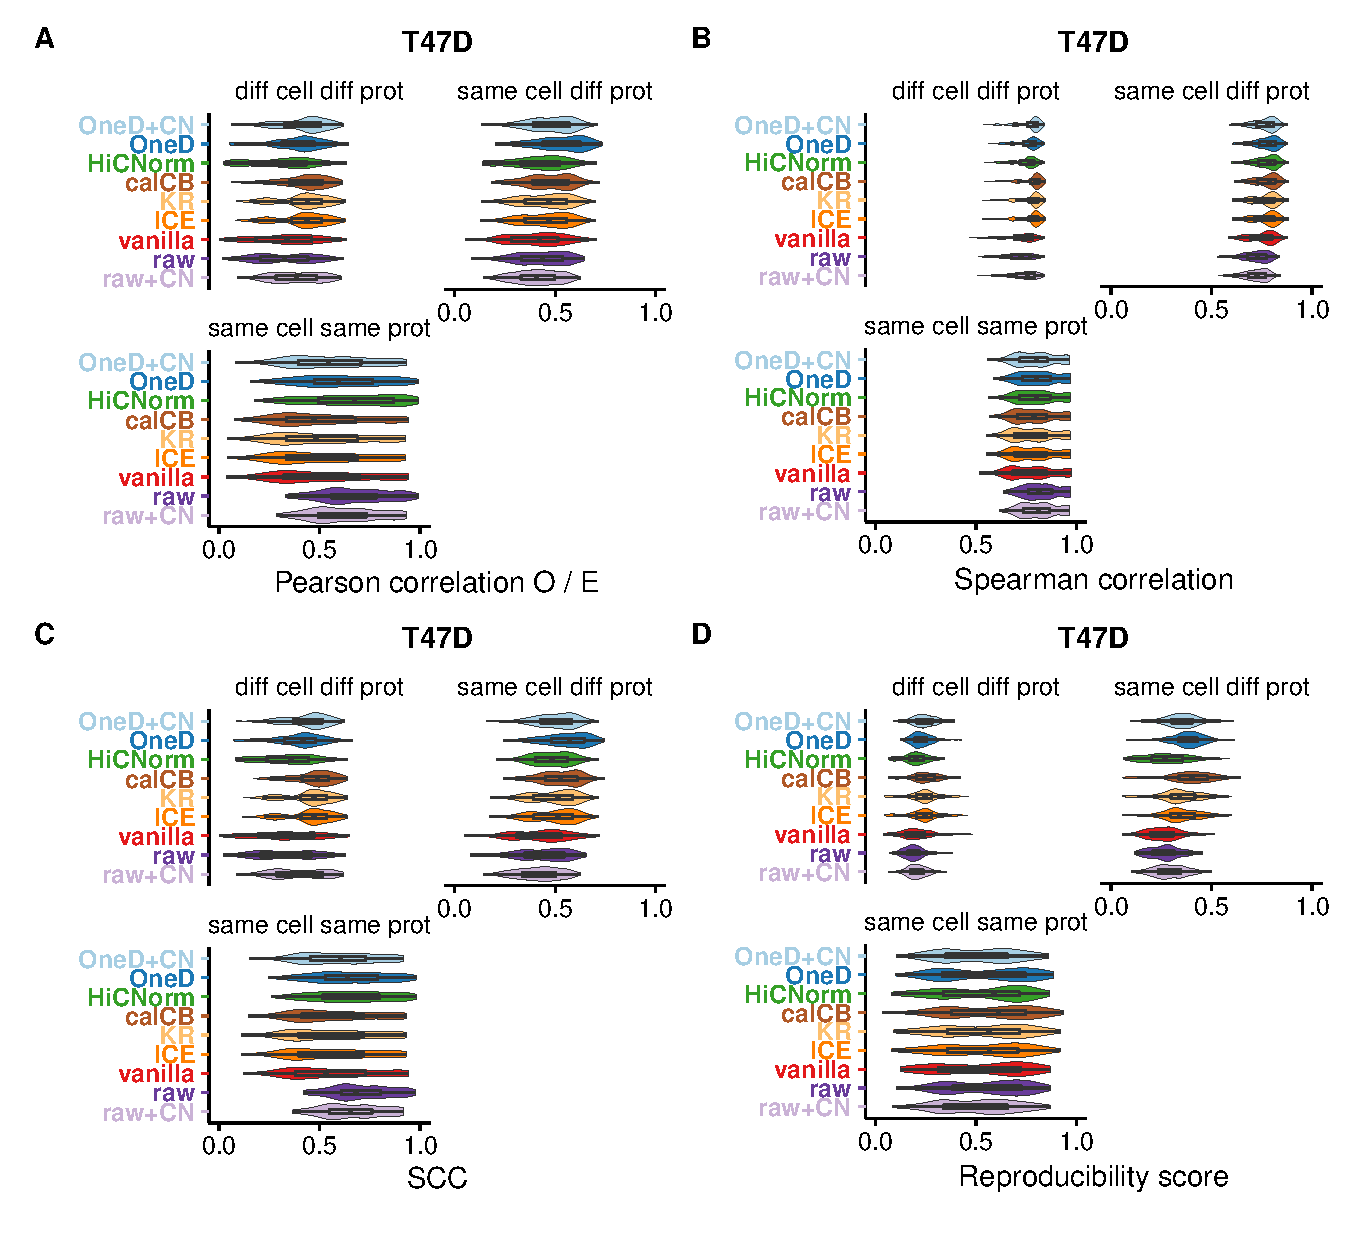
\includegraphics[width=\textwidth]{nar_figures/supp_figure_2.eps}}
    \caption{
    Distribution of the pair-wise comparisons between the samples included in
    the T47D set. X axis: similarity metric. Y axis: correction
    method. Each panel groups pairs of samples with the corresponding
    characteristics (in terms of cell type and protocol). A. Pearson correlation
    between observed over expected counts. B. Spearman correlation between
    observed counts. C. Stratum-adjusted correlation coefficient (SCC) between
    observed counts. D. Reproducibility score of observed counts.}
\end{figure}

\begin{figure}
	\centerline{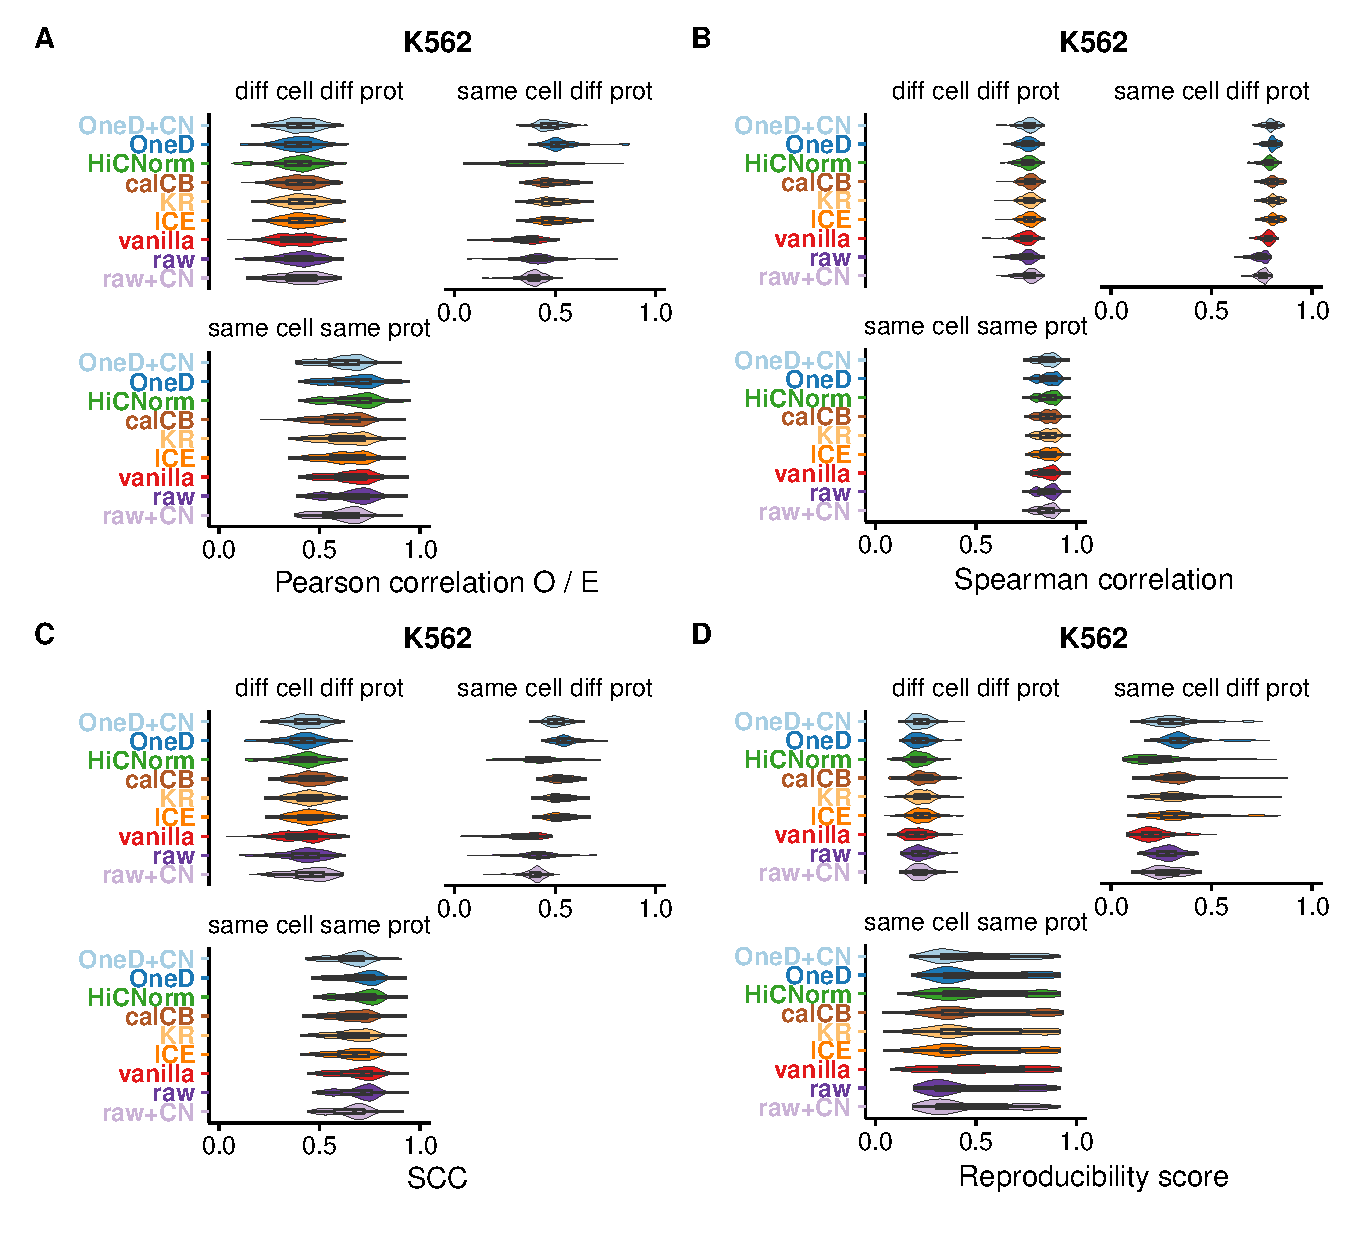
\includegraphics[width=\textwidth]{nar_figures/supp_figure_3.eps}}
    \caption{
    Distribution of the pair-wise comparisons between the samples included in
    the K562 set. X axis: similarity metric. Y axis: correction
    method. Each panel groups pairs of samples with the corresponding
    characteristics (in terms of cell type and protocol). A. Pearson correlation
    between observed over expected counts. B. Spearman correlation between
    observed counts. C. Stratum-adjusted correlation coefficient (SCC) between
    observed counts. D. Reproducibility score of observed counts.}
\end{figure}

\begin{figure}
	\centerline{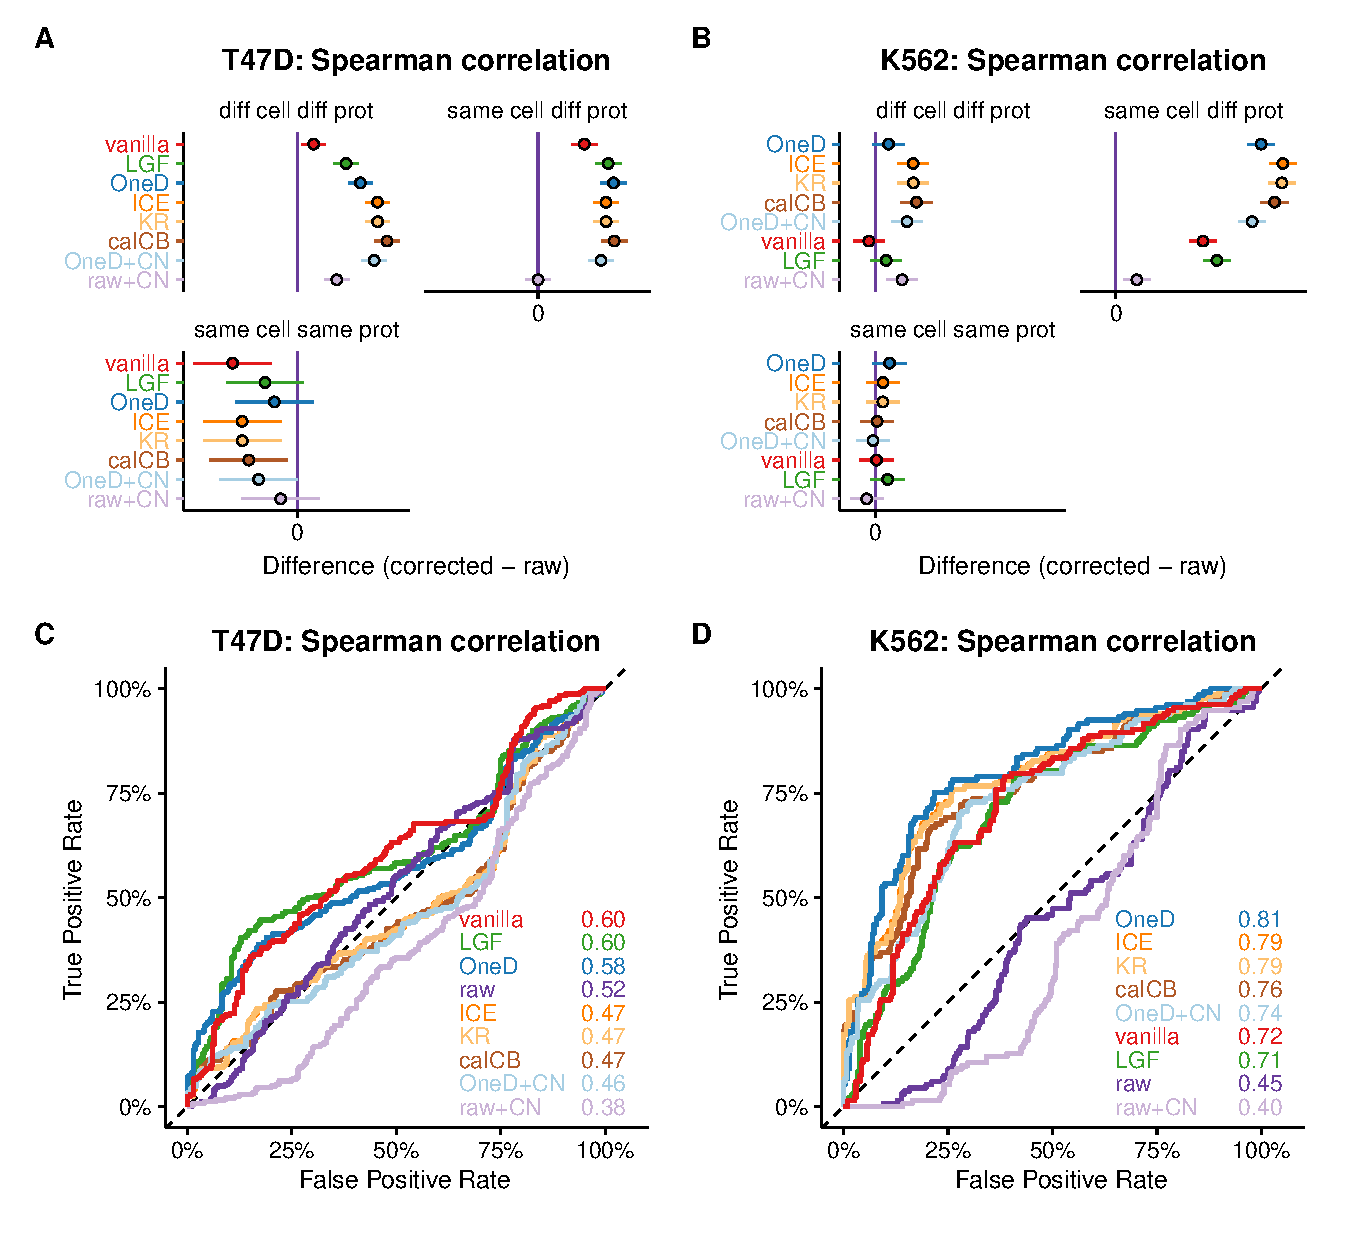
\includegraphics[width=\textwidth]{nar_figures/supp_figure_4.eps}}
    \caption{
    Removing biases from Hi-C on aberrant karyotypes (Spearman correlation). A and B. Average changes
    compared to the raw data on the T47D and K562 data sets. The bars represent
    95\% confidence intervals centered on the mean difference of the
    spearman correlation between a given correction method and the raw data. C
    and D. ROC curves on the T47D and K562 sets. The areas under the curve are
    indicated in the bottom right corner. The color code is the same as in panels A and B.}
\end{figure}

\begin{figure}
	\centerline{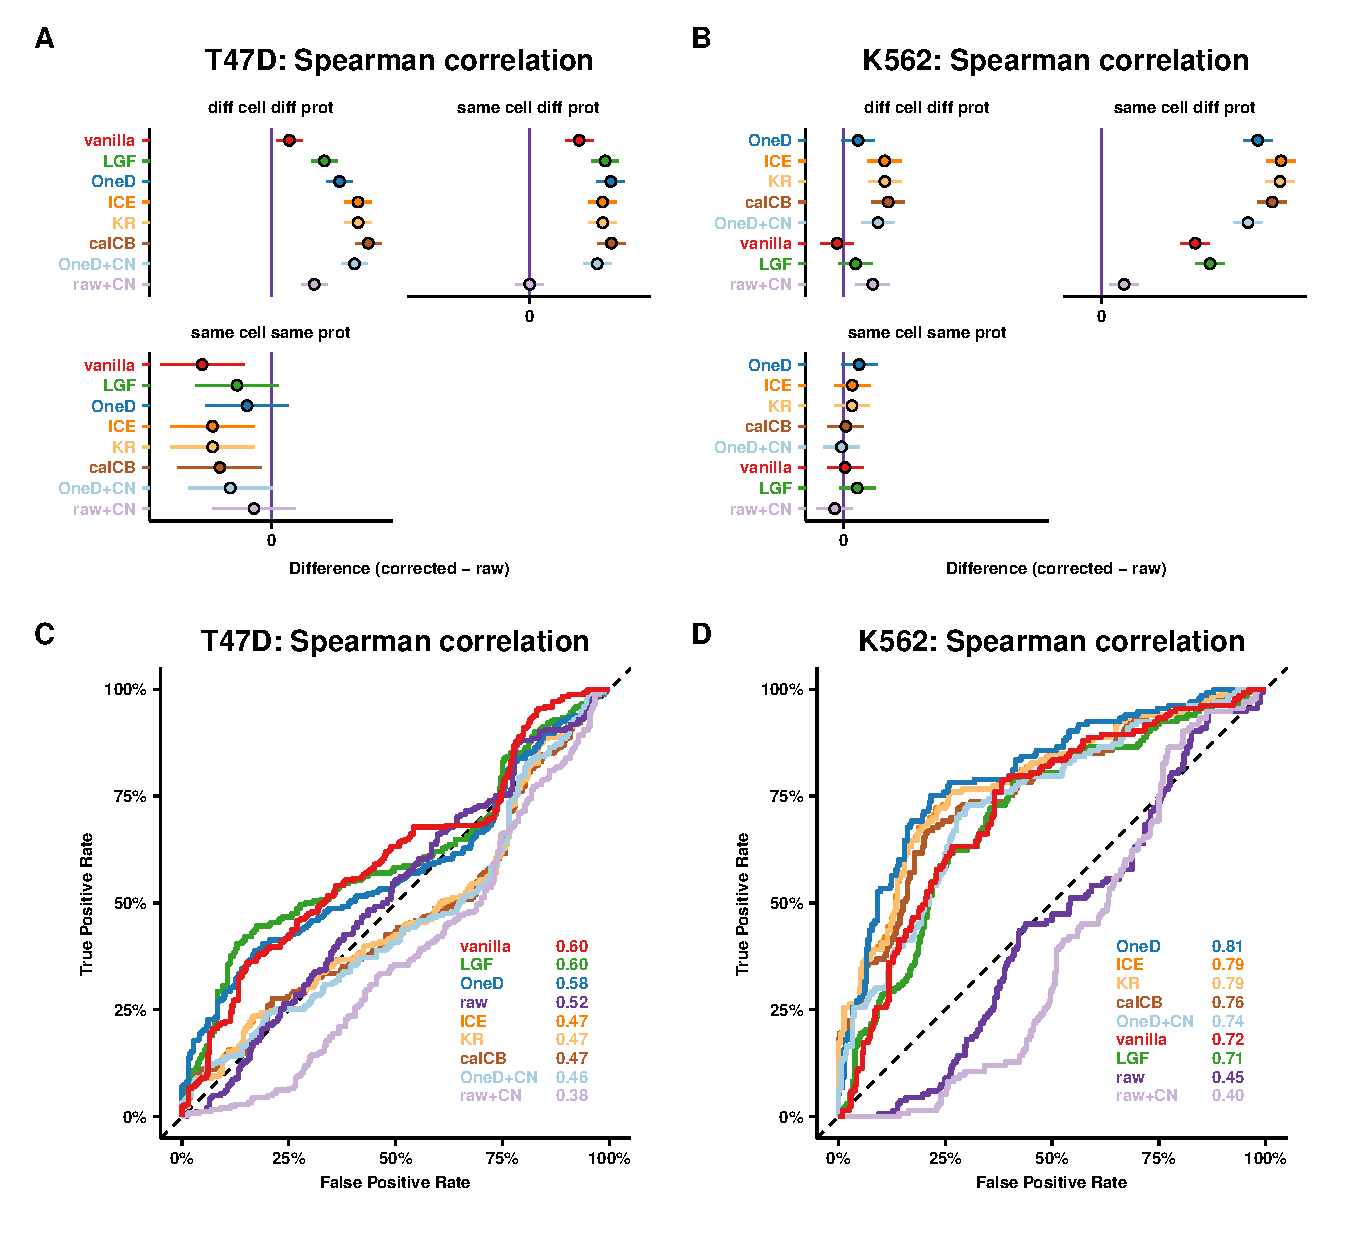
\includegraphics[width=\textwidth]{nar_figures/supp_figure_5.eps}}
    \caption{
    Removing biases from Hi-C on aberrant karyotypes (Pearson correlation). A and B. Average changes
    compared to the raw data on the T47D and K562 data sets. The bars represent
    95\% confidence intervals centered on the mean difference of the
    Pearson correlation of the observed over expected between a given correction method and the raw data. C
    and D. ROC curves on the T47D and K562 sets. The areas under the curve are
    indicated in the bottom right corner. The color code is the same as in panels A and B.}
\end{figure}

\begin{figure}
	\centerline{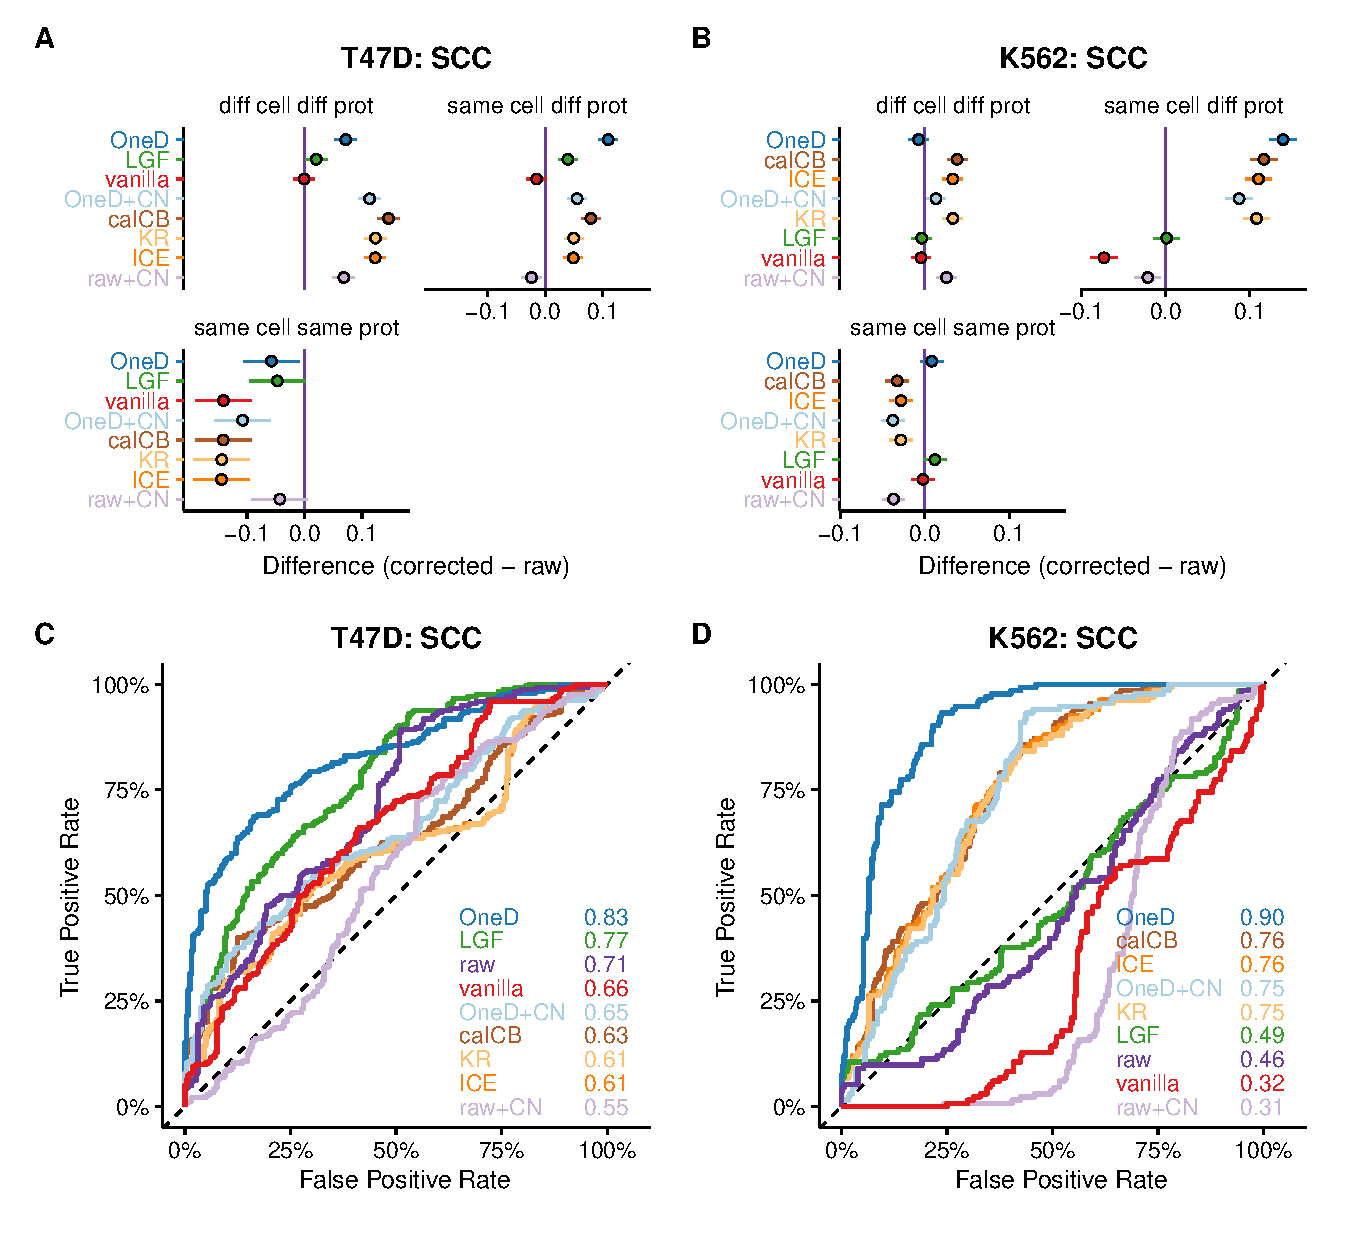
\includegraphics[width=\textwidth]{nar_figures/supp_figure_6.eps}}
    \caption{
    Removing biases from Hi-C on aberrant karyotypes (SCC). A and B. Average changes
    compared to the raw data on the T47D and K562 data sets. The bars represent
    95\% confidence intervals centered on the mean difference of the
    stratum-adjusted correlation coefficient (SCC) between a given correction method and the raw data. C
    and D. ROC curves on the T47D and K562 sets. The areas under the curve are
    indicated in the bottom right corner. The color code is the same as in panels A and B.}
\end{figure}

\begin{figure}
	\centerline{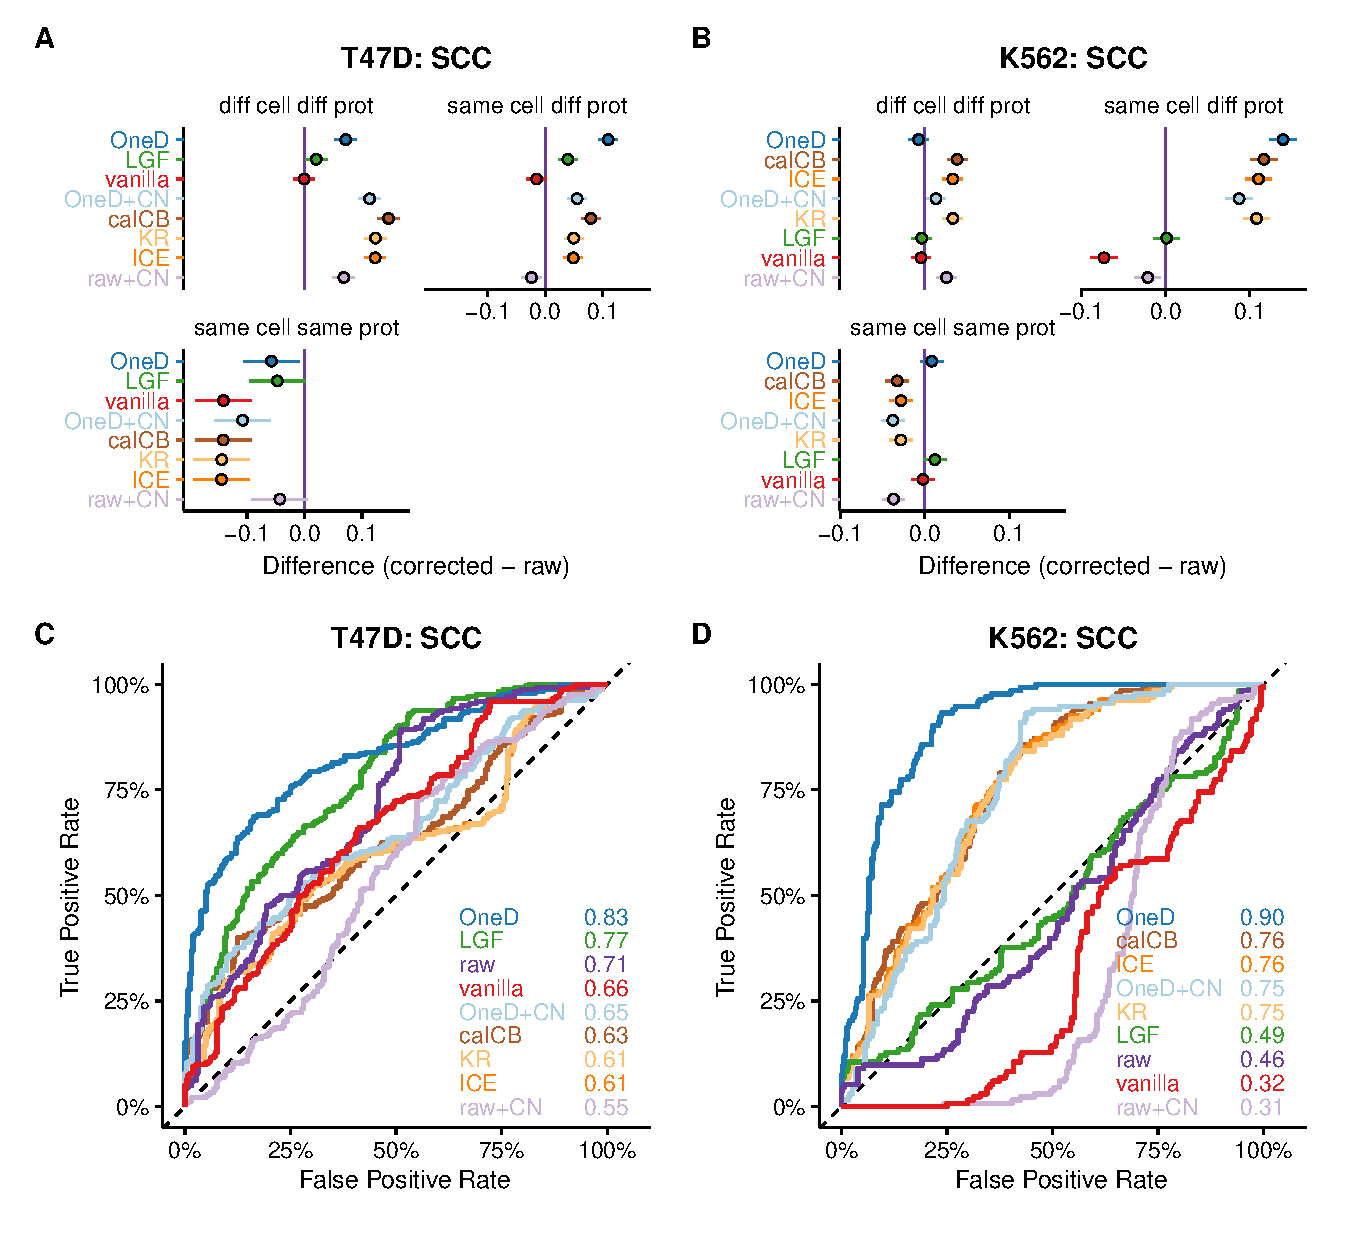
\includegraphics[width=\textwidth]{nar_figures/supp_figure_7.eps}}
    \caption{
    Distribution of the pair-wise comparisons between the samples included in
    the mm10 set. X axis: similarity metric. Y axis: correction
    method. Each panel groups pairs of samples with the corresponding
    characteristics (in terms of cell type and protocol). A. Pearson correlation
    between observed over expected counts. B. Spearman correlation between
    observed counts. C. Stratum-adjusted correlation coefficient (SCC) between
    observed counts. D. Reproducibility score of observed counts.}
\end{figure}

\begin{figure}
	\centerline{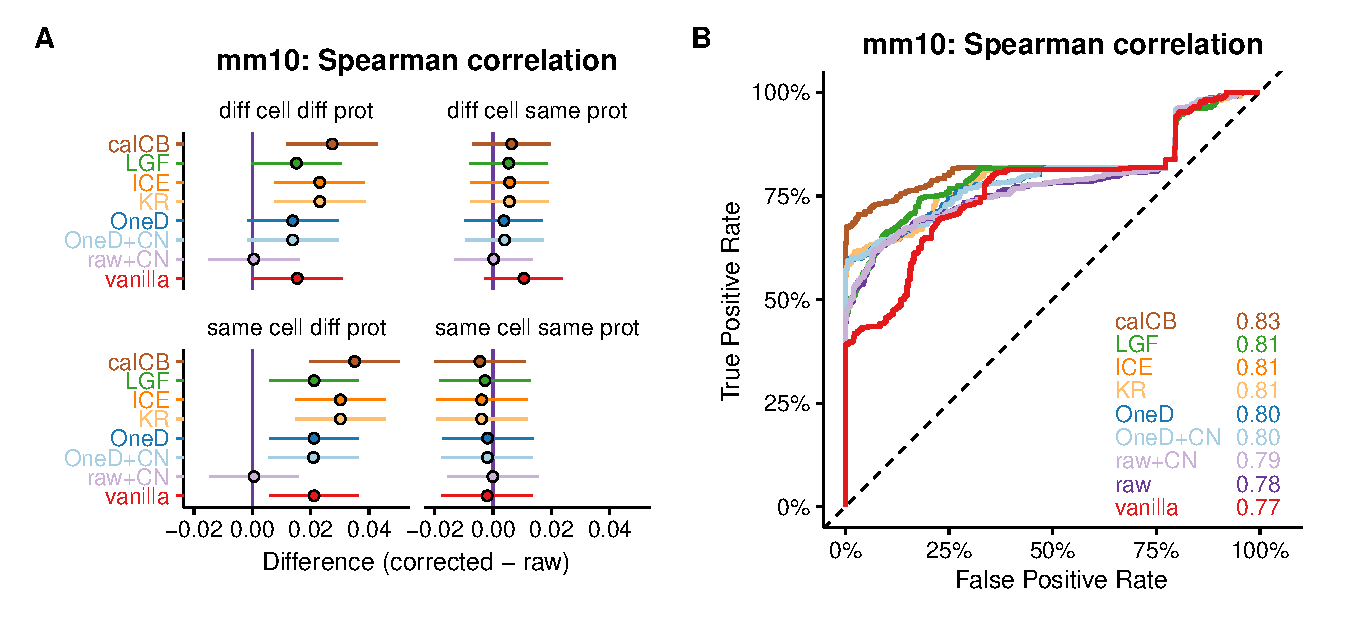
\includegraphics[width=\textwidth]{nar_figures/supp_figure_8.eps}}
    \caption{
    Removing biases from Hi-C on normal karyotypes (Spearman correlation). A. Average changes
    compared to the raw data on the mm10 data set. The bars represent
    95\% confidence intervals centered on the mean difference of the
    Spearman correlation between a given correction method and the raw
    data. B. ROC curves on the mm10 set. The areas under the curve are indicated
    in the bottom right corner. The color code is the same as in panel A.}
\end{figure}

\begin{figure}
	\centerline{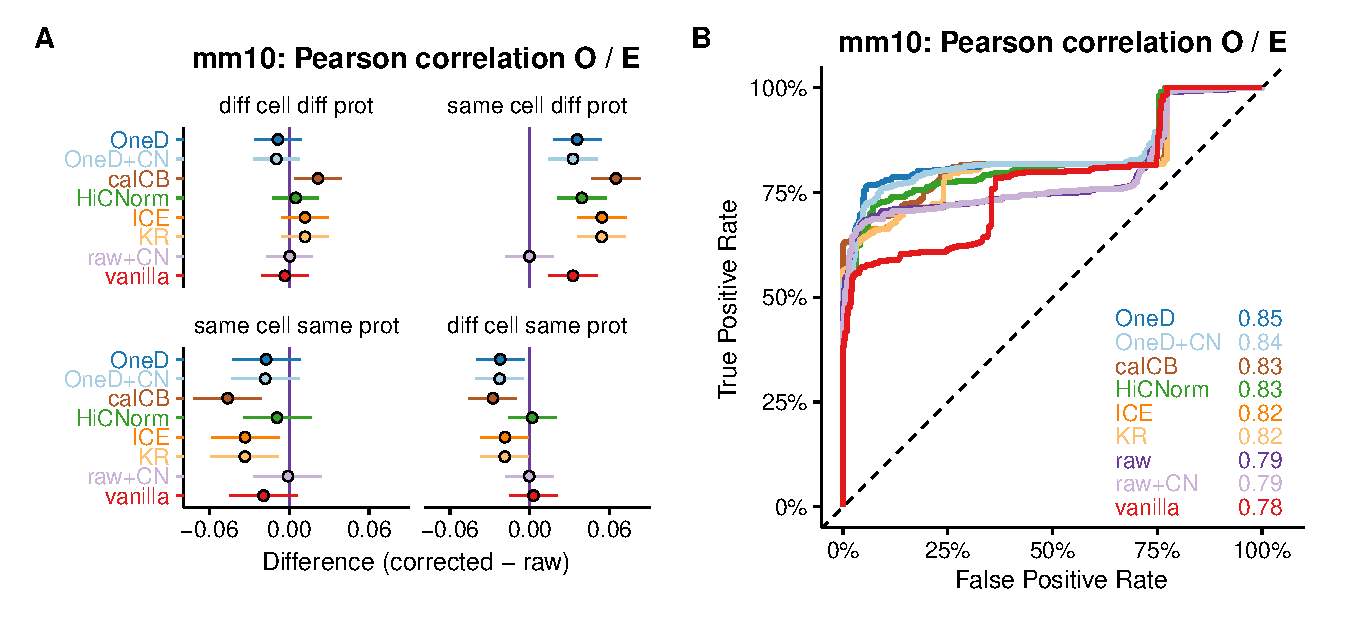
\includegraphics[width=\textwidth]{nar_figures/supp_figure_9.eps}}
    \caption{
    Removing biases from Hi-C on normal karyotypes (Pearson correlation). A. Average changes
    compared to the raw data on the mm10 data set. The bars represent
    95\% confidence intervals centered on the mean difference of the
    Pearson correlation of the observed over expected correlation between a given correction method and the raw
    data. B. ROC curves on the mm10 set. The areas under the curve are indicated
    in the bottom right corner. The color code is the same as in panel A.}
\end{figure}

\begin{figure}
	\centerline{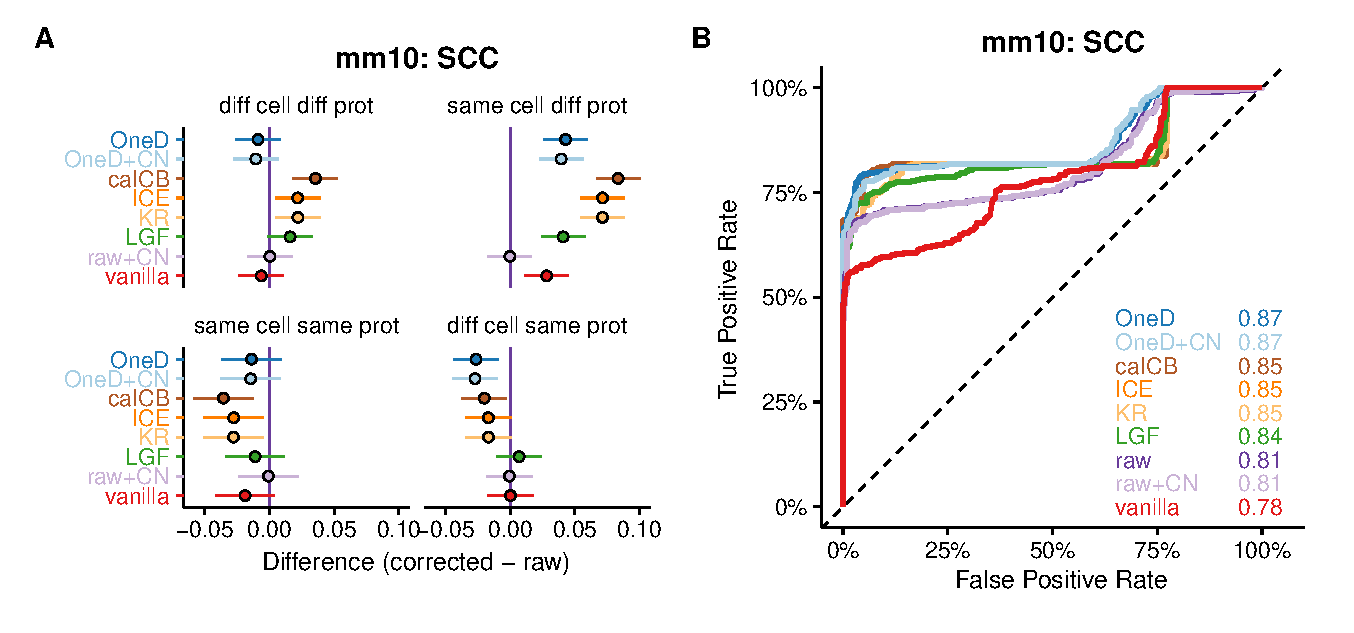
\includegraphics[width=\textwidth]{nar_figures/supp_figure_10.eps}}
    \caption{
    Removing biases from Hi-C on normal karyotypes (SCC). A. Average changes
    compared to the raw data on the mm10 data set. The bars represent
    95\% confidence intervals centered on the mean difference of the
    stratum-adjusted correlation coefficient (SCC) between a given correction method and the raw
    data. B. ROC curves on the mm10 set. The areas under the curve are indicated
    in the bottom right corner. The color code is the same as in panel A.}
\end{figure}

\begin{figure}
	\centerline{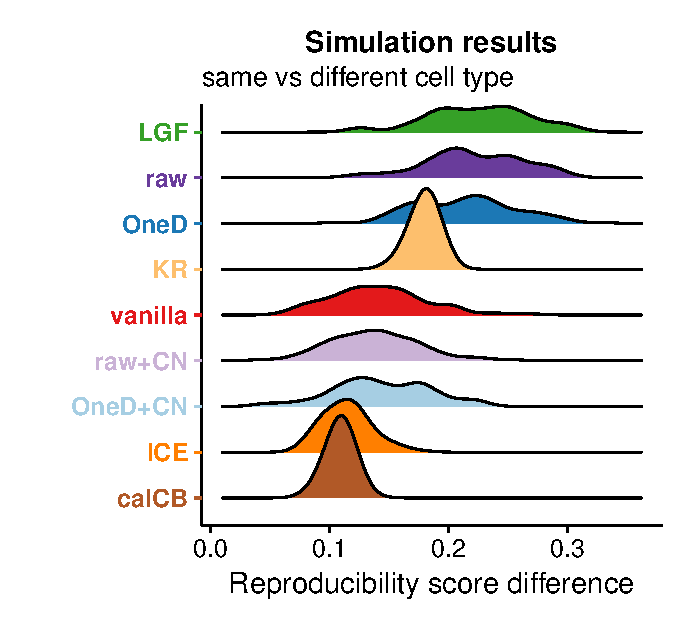
\includegraphics[width=\textwidth]{nar_figures/supp_figure_11.eps}}
    \caption{
    Removing biases from Hi-C on GM12878 samples. X axis: reproducibility
    score. Y axis: correction method. The bars represent 95\% confidence intervals centered on the mean of the
    reproducibility score of each correction method. The vertical dark purple
    line marks the reproducibility score for the uncorrected data (raw). Upper panel: pairs of
    samples processed using different protocols. Lower panel: pairs of samples
    processed using the same protocol.}
\end{figure}

\begin{figure}
	\centerline{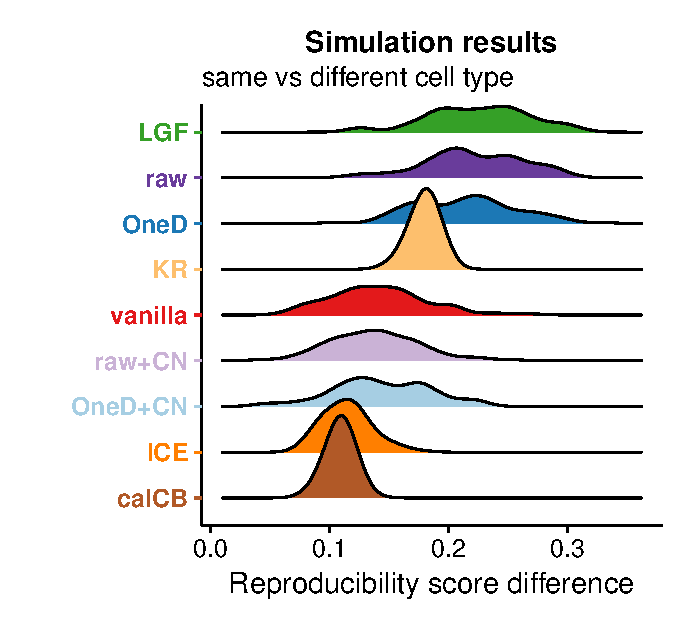
\includegraphics[width=\textwidth]{nar_figures/supp_figure_12.eps}}
    \caption{
    Distribution of the simulation results. X axis: Difference in
    reproducibility score between pairs of samples of the same cell type and
    pairs of samples of different cell type. Y axis: correction method}
\end{figure}

\begin{figure}
	\centerline{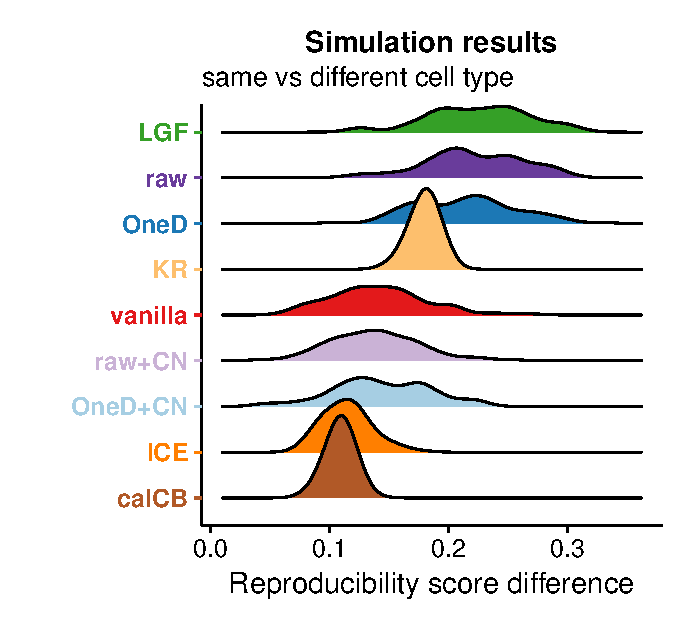
\includegraphics[width=\textwidth]{nar_figures/supp_figure_13.eps}}
    \caption{Correlation between subsamples at different resolutions and
    depths. X axis: sequencing depth. Y axis: Pearson correlation between the
    correction vectors of two different subsamples. Each color represents a
    correction method and each panel a bining resolution. Note the Y axis limits
    are specific to each panel.}
\end{figure}


\end{document}
